\documentclass[sigconf,nonacm,screen]{acmart}
\usepackage{filecontents}
\usepackage{textcomp}
\usepackage{pgfplots}
\usetikzlibrary{patterns}
\usepackage{ifthen}
\usepgfplotslibrary{groupplots}
\RequirePackage{keyval}
\usepackage{multirow}
\usepackage{multicol}
\usepackage{csvsimple}
\usepackage[utf8]{inputenc}
\newcounter{row}
\newcounter{col}
\usepackage{wrapfig}
\usepackage{textgreek}
\usepackage[inline]{enumitem}
% \usepackage[table]{xcolor}
\usetikzlibrary{matrix, positioning}
\usetikzlibrary{patterns,tikzmark}
\usetikzlibrary{matrix,decorations.pathreplacing,calc}
\usepackage{hf-tikz}
\usepackage{pifont}
\usepackage{subfig}
\usetikzlibrary{chains,fit,shapes}
\usetikzlibrary{arrows.meta,
    chains,
    positioning,
    shapes.symbols}
\usetikzlibrary{decorations,calligraphy}
\usepackage{pgfplotstable}
\usepgfplotslibrary{statistics}
%\pgfplotsset{compat=newest}
\usetikzlibrary{matrix,calc}
\usetikzlibrary{fit}
\usepackage{xfp}
\usepackage{mathtools}

\usetikzlibrary{positioning}

\usepackage{makecell}
%\usepackage{tabu}
\usepackage{tikz}
\usetikzlibrary{trees}

%\pgfplotsset{compat=1.8}
\pgfplotsset{compat=1.12}


\usepgfplotslibrary{fillbetween}

\usepackage{filecontents}
% \usetikzlibrary{pgfplots.groupplots}
% \pgfplotsset{compat=1.9}

% \usepackage[utf8]{inputenc}
% \usepackage[ngerman]{babel}
% \usepackage{pgfplots}
% \pgfplotsset{compat=1.9}
% \usetikzlibrary{
%   pgfplots.groupplots,
%   matrix
% }
% \usepackage{siunitx}

\newtheorem{theorem}{Theorem}
\newtheorem{definition}{Definition}
\newcommand{\eat}[1]{}

\definecolor{bluegreen}{RGB}{3, 166, 155}
\definecolor{pitchblack}{RGB}{0, 0, 0}
\definecolor{lightbeige}{RGB}{255, 251, 241}
\definecolor{mediumgray}{RGB}{183, 183, 183}
\definecolor{mygreen}{rgb}{0,0.6,0}
\definecolor{mygray}{rgb}{0.5,0.5,0.5}
\definecolor{mymauve}{rgb}{0.58,0,0.82}
\definecolor{keywords}{RGB}{255,0,90}
\definecolor{comments}{RGB}{0,0,113}
\definecolor{red}{RGB}{255,0,0}
\definecolor{green}{RGB}{0,255,0}
\definecolor{navy}{RGB}{0,0,128}
\definecolor{DarkGrenen}{RGB}{0,100,0}
\definecolor{DarkOliveGreen}{RGB}{85,107,47}
\definecolor{saddlebrown}{RGB}{139,69,19}
\definecolor{gold}{RGB}{252,194,1}
\definecolor{tug}{RGB}{247,1,70}
\definecolor{tugb}{RGB}{120,137,251}

\definecolor{color01}{RGB}{159,96,0}
\definecolor{color02}{RGB}{43,85,128}


\definecolor{blue0}{RGB}{153,153,153}
\definecolor{blue1}{RGB}{77,77,77}%
\definecolor{blue2}{RGB}{165,71,209}
\definecolor{blue3}{RGB}{77,10,142}
\definecolor{blue4}{RGB}{74,139,203}
\definecolor{blue5}{RGB}{40,40,190}

\definecolor{color1}{RGB}{100,149,237} % corn flower blue
\definecolor{color2}{RGB}{153,153,153} % light gray
\definecolor{color3}{RGB}{0,0,0} % black
\definecolor{color4}{RGB}{255,165,0} % orange
\definecolor{color5}{RGB}{255,69,0} % orange red
\definecolor{color6}{RGB}{77,77,77} % dark gray
\definecolor{color7}{RGB}{31,119,180}
\definecolor{color8}{RGB}{7,77,125}
\definecolor{color9}{RGB}{153,216,201}


\definecolor{teal1}{RGB}{31, 111, 111}
\definecolor{teal2}{RGB}{84, 161, 161}
\definecolor{teal3}{RGB}{159, 200, 200}

\definecolor{dred1}{RGB}{160, 0, 0}
\definecolor{dred2}{RGB}{196, 102, 102}
\definecolor{dred3}{RGB}{216, 166, 166}


\definecolor{dblue1}{RGB}{32, 102, 168}
\definecolor{dblue2}{RGB}{53, 148, 204}
\definecolor{dblue3}{RGB}{140, 197, 227}

\definecolor{totalcolor}{RGB}{2, 152, 215}
\definecolor{mvcolor}{RGB}{248, 163, 47}
\definecolor{dvcolor}{RGB}{203, 70, 39}



% Enable this two commands when you want to extract diagrams in extra files, then run "make"
\usetikzlibrary{external}
\tikzexternalize[prefix=plots/] %  activate

\usetikzlibrary{positioning}

\sloppy
\clubpenalty = 10000
\widowpenalty = 10000
\brokenpenalty = 10000
\frenchspacing


\makeatletter
\def\pgfplots@drawaxis@lines@preparediscont@for#1{%
        \ifnum\csname pgfplots@#1axisdiscontnum\endcsname>0
                \begingroup
                % this group employs several temporary dimension registers
                % and is therefor scoped:
                \let\disstart=\pgf@ya
                \let\disend=\pgf@yb
                \disend=\csname pgfplots@#1max@reg\endcsname
                \advance\disend by -\csname pgfplots@#1min@reg\endcsname
                \disend=\csname pgfplots@#1@veclength\endcsname\disend
                \ifcase\csname pgfplots@#1axisdiscontnum\endcsname\relax
                        % has already been checked above.
                \or
                        \def\discontstyle{decoration={zigzag,segment length=5pt, amplitude=2pt}}%
                        \advance \disend by -8pt
                \or
                        \def\discontstyle{decoration={ticks,segment length=4pt, amplitude=8pt}}%
                        \advance \disend by -4pt
                \fi
                \pgfplotscoordmath{#1}{datascaletrafo get params}%
                % if #1max + shift < 0pt  (shift is 0 without the scaling trafo)
                \ifdim\csname pgfplots@#1max@reg\endcsname<-\pgfplotsretvalb pt
                        % swap start and end
                        \disstart=\disend
                        \disend=2pt
                \else
                        \disstart=2pt
                \fi
                % carry local computations outside of group:
                \xdef\pgfplots@glob@TMPa{%
                        \noexpand\def\expandafter\noexpand\csname #1disstart\endcsname{\the\disstart}%
                        \noexpand\def\expandafter\noexpand\csname #1disend\endcsname{\the\disend}%
                        \noexpand\pgfkeysdef{/tikz/#1discont}{\noexpand\pgfkeysalso{\discontstyle}}%
                }%
                \endgroup
                \pgfplots@glob@TMPa
        \else
                \expandafter\def\csname #1disstart\endcsname{0pt}%
                \expandafter\def\csname #1disend\endcsname{0pt}%
                \pgfkeyslet{/tikz/#1discont}=\pgfutil@empty
        \fi
}%
\makeatother



\begin{document}
\title[Query Processing by Data Catalog]{Query Processing by Data Catalog}

\author{Saeed Fathollahzadeh} 
\orcid{0000-0003-3723-6191}
\affiliation{
\institution{Concordia University}
\country{Canada}}

\renewcommand{\shortauthors}{Saeed Fathollahzadeh}

\maketitle
    
    % \tikzsetnextfilename{Experiment5-Utility-MV} 
    %     \begin{figure}[!ht]
    %         \centering
    %         \input{Experiment5/Experiment5-Utility-MV.tex}
    %         \caption{Experiment5-Utility-MV}
    %     \end{figure}  

    % \tikzsetnextfilename{Experiment5-Utility-OUT} 
    %     \begin{figure}[!ht]
    %         \centering
    %         \input{Experiment5/Experiment5-Utility-OUT.tex}
    %         \caption{Experiment5-Utility-OUT}
    %     \end{figure}      

    %     \tikzsetnextfilename{Experiment5-Utility-MVOUT} 
    %     \begin{figure}[!ht]
    %         \centering
    %         \begin{tikzpicture}
  \newcommand{\myaddplotds}[3]{ 
    \addplot[color=#2,mark=#3, line width=0.7pt] 
    table[y=Result, col sep=comma, x=MV, discard if singlconfig={0.05}{gemini-1.5-pro-latest}{#1}{Utility}]
    {../archive/VLDB2025/results/EtoEResults.csv};
    \label{#1}  
   
  };


\pgfplotsset{
    discard if singlconfig/.style n args={4}{
        x filter/.code={
            \edef\tempa{\thisrow{OUT}}
            \edef\tempb{#1}
            \ifx\tempa\tempb
              \edef\tempc{\thisrow{llm_model}}
                \edef\tempd{#2}
                  \ifx\tempc\tempd  
                  %
                    \edef\tempe{\thisrow{Config}} 
                    \edef\tempf{#3}
                    \ifx\tempe\tempf 
                    %
                    \edef\tempg{\thisrow{dataset_name}} 
                    \edef\temph{#4}
                    \ifx\tempg\temph 
        
                    \else
                    \def\pgfmathresult{inf}
                    \fi
                    %
                    \else
                    \def\pgfmathresult{inf}
                  \fi
                  %                
                  \else
                  \def\pgfmathresult{inf}
                  \fi
            \else
            \def\pgfmathresult{inf}
            \fi			
        }
    },
};   

\begin{axis}[
  ymin=-0.2,
  ymax=1,
  %xmax=0.05,
  y tick label style={/pgf/number format/1000 sep={}},
  x tick label style={/pgf/number format/1000 sep={}},  
  scaled x ticks=false,
  axis line style={black, line width=0.3pt},
  enlarge y limits={0.06,upper},
  enlarge x limits=0.05,
  ylabel={$R^2$ $\%$},
  xlabel={Missing Percentage [\%]},
  log ticks with fixed point,
  xtick align=outside,
  xtick pos=left,
  ytick pos=left,
  yticklabel style = {font=\large},
  ylabel style = {font=\large, yshift=-6pt, xshift=-3pt},
  height=.5\columnwidth,
  width=0.55\columnwidth,
  grid=both,
  grid style=dotted,
  minor grid style={gray!70},
  every axis plot/.append style={line width=0.7pt,mark options={scale=1,solid, line width=0.7pt}},  
  xticklabel style = {font=\normalsize, xshift=0pt, yshift=2pt},
  legend image post style={line width=.5pt},          
  bar width=8pt,         
  ytick={-0.15,0,0.2, 0.4, 0.6, 0.8, 1},
  yticklabels={Fail,0, 20, 40, 60, 80, 100},               
  xtick={0, 0.1, 0.2, 0.3, 0.4, 0.5},
  xticklabels={0, 10, 20, 30, 40, 50},  
]
\myaddplotds{CatDB}{tug}{square*};
\myaddplotds{CAAFE}{teal1}{diamond*};
\myaddplotds{Flaml}{color4}{square*};
\myaddplotds{Autogluon}{dblue1}{triangle*};
\myaddplotds{AutoSklearn}{black}{o};
\myaddplotds{H2O}{tugb}{triangle};

\draw[gray, thick,densely dotted] (axis cs:-0.1,0) -- (axis cs:1,0);
\end{axis}

% \node [draw=none,inner sep=0, font=\footnotesize, anchor=west] (leg1) at (rel axis cs: 0.06,0.87) {\shortstack[l]{
%   \ref{CatDBChain} CatDB Chain \ \ \ref{Autogluon} Autogluon \ \ \ref{H2O} H2O\\
%   \ref{AutoSklearn} AutoSklearn \ \ref{Flaml} Flaml \ \ref{CAAFE} CAAFE R.F.}};

\end{tikzpicture}
    %         \caption{Experiment5-Utility-MVOUT}
    %     \end{figure}      

    % \tikzsetnextfilename{Experiment5-Volkert-OUT} 
    % \begin{figure}[!ht]
    %     \centering
    %     \input{Experiment5/Experiment5-Volkert-OUT.tex}
    %     \caption{Experiment5-Volkert-OUT}
    % \end{figure}     

    % \tikzsetnextfilename{Experiment5-Volkert-MV} 
    % \begin{figure}[!ht]
    %     \centering
    %     \input{Experiment5/Experiment5-Volkert-MV.tex}
    %     \caption{Experiment5-Volkert-MV}
    % \end{figure}  
    
    % \tikzsetnextfilename{Experiment5-Volkert-MVOUT} 
    % \begin{figure}[!ht]
    %     \centering
    %     \input{Experiment5/Experiment5-Volkert-MVOUT.tex}
    %     \caption{Experiment5-Volkert-MVOUT}
    % \end{figure}  

    \tikzsetnextfilename{Experiment5-Legend} 
    \begin{figure}[!ht]
        \centering
        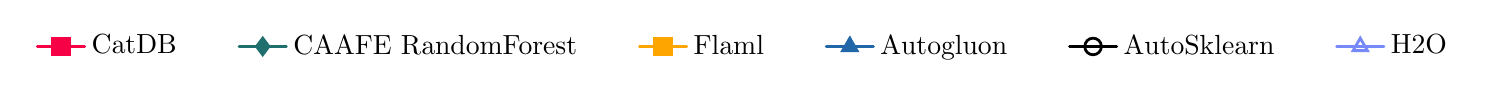
\begin{tikzpicture} 
  \begin{axis}[%
  hide axis,
  xmin=10,
  xmax=50,
  ymin=0,
  ymax=0.4, 
  legend columns=6,
  legend style={draw=white!15!black,legend cell align=left},
  legend style={draw=none, nodes={scale=1, inner ysep=0.2mm, transform shape,}, font=\normalsize},    
  legend image post style={line width=1pt,scale=1},
  legend cell align={left},   
  /tikz/every even column/.append style={column sep=2em, row sep=0.5em},
  %legend image code/.code={\draw [#1] (0cm,-0.12cm) rectangle (0.2cm,0.12cm); }, 
  ]
  \addlegendimage{tug,draw=tug, fill=tug,line width=0.3pt, mark=square*, line cap=round,mark options={scale=1.5,solid}}
  \addlegendentry{CatDB};

  \addlegendimage{teal1,draw=teal1, fill=teal1,line width=0.3pt, mark=diamond*, line cap=round,mark options={scale=1.5,solid}}
  \addlegendentry{CAAFE RandomForest};

  \addlegendimage{color4,draw=color4, fill=color4,line width=0.3pt, mark=square*, line cap=round,mark options={scale=1.5,solid}}
  \addlegendentry{Flaml};

  \addlegendimage{dblue1,draw=dblue1, fill=dblue1,line width=0.3pt, mark=triangle*, line cap=round,mark options={scale=1.5,solid}}
  \addlegendentry{Autogluon};

  \addlegendimage{black,draw=black, fill=black,line width=0.3pt, mark=o, line cap=round,mark options={scale=1.5,solid}}
  \addlegendentry{AutoSklearn};

  \addlegendimage{tugb,draw=tugb, fill=tugb,line width=0.3pt, mark=triangle, line cap=round,mark options={scale=1.5,solid}}
  \addlegendentry{H2O};
  
  \end{axis}  
\end{tikzpicture}

        \caption{Experiment5-Legend}
    \end{figure}

    

    % \tikzsetnextfilename{Experiment4-NYC-MV} 
    %     \begin{figure}[!ht]
    %         \centering
    %         \begin{tikzpicture}

  \newcommand{\myaddplotds}[3]{ 
    \addplot[color=#2,mark=#3, line width=0.3pt] 
    table[y=Result, col sep=comma, x=MV, discard if singlconfig={0.0}{gemini-1.5-pro-latest}{#1}]
    {../archive/SIGMOD2025-Results/EtoE/EtoEResults.csv};
    \label{#1}  
   
  };


\pgfplotsset{
    discard if singlconfig/.style n args={3}{
        x filter/.code={
            \edef\tempa{\thisrow{OUT}}
            \edef\tempb{#1}
            \ifx\tempa\tempb
              \edef\tempc{\thisrow{llm_model}}
                \edef\tempd{#2}
                  \ifx\tempc\tempd  
                  %
                    \edef\tempe{\thisrow{Config}} 
                    \edef\tempf{#3}
                    \ifx\tempe\tempf 
        
                    \else
                    \def\pgfmathresult{inf}
                  \fi
                  %                
                  \else
                  \def\pgfmathresult{inf}
                  \fi
            \else
            \def\pgfmathresult{inf}
            \fi			
        }
    },
};   

\begin{axis}[
  ymin=0,
  ymax=1,
  % ybar stacked,
  y tick label style={/pgf/number format/1000 sep={}},
  x tick label style={/pgf/number format/1000 sep={}},  
  scaled y ticks=false,
  axis line style={black, line width=0.3pt},
  enlarge y limits={0.3,upper},
  enlarge x limits=0.1,
  ylabel={AUC-ovr $\%$},
  xlabel={Missing Percentage},
  log ticks with fixed point,
  xtick align=outside,
  xtick pos=left,
  ytick pos=left,
  yticklabel style = {font=\large},
  ylabel style = {font=\large, yshift=0pt, xshift=-3pt},
  height=.6\columnwidth,
  width=1\columnwidth,
  ymajorgrids=true,
  grid style=dotted,
  minor grid style={gray!70},
  %nodes near coords,
  %every node near coord/.append style={font=\fontsize{0.1pt}{0.1}, rotate=90, xshift=8pt, yshift=0pt},
  every axis plot/.append style={line width=0.4pt,mark options={scale=1.5,solid}},  
  xticklabel style = {font=\normalsize, xshift=0pt, yshift=2pt},
  legend image post style={line width=.5pt},          
  bar width=8pt,         
  ytick={0,0.2, 0.4, 0.6, 0.8, 1},
  yticklabels={0, 20, 40, 60, 80, 100},               
  %every x tick/.style={ draw=none},
  %xtick = data,
  xtick={0, 0.1, 0.2, 0.3, 0.4, 0.5},
  xticklabels={Original Data,$10\%$, $20\%$, $30\%$, $40\%$, $50\%$},  
  %legend image code/.code={\draw [#1] (0cm,-0.1cm) rectangle (0.25cm,0.1cm); }, 
]
\myaddplotds{CatDB}{tug}{square*};
\end{axis}

\node [draw=none,inner sep=0, font=\normalsize, anchor=west] (leg1) at (rel axis cs: 0.1,0.9) {\shortstack[l]{
  \ref{CatDB} CatDB}};

\end{tikzpicture}
    %         \caption{Experiment4-NYC-MV}
    %     \end{figure}  
        
    % \tikzsetnextfilename{Experiment4-NYC-OUT} 
    %     \begin{figure}[!ht]
    %         \centering
    %         \begin{tikzpicture}
  \newcommand{\myaddplotds}[3]{ 
    \addplot[color=#2,mark=#3, line width=0.7pt] 
    table[y=Result, col sep=comma, x=OUT, discard if singlconfig={0.0}{gemini-1.5-pro-latest}{#1}]
    {../archive/SIGMOD2025-Results/EtoE/EtoEResults.csv};
    \label{#1}  
   
  };


\pgfplotsset{
    discard if singlconfig/.style n args={3}{
        x filter/.code={
            \edef\tempa{\thisrow{MV}}
            \edef\tempb{#1}
            \ifx\tempa\tempb
              \edef\tempc{\thisrow{llm_model}}
                \edef\tempd{#2}
                  \ifx\tempc\tempd  
                  %
                    \edef\tempe{\thisrow{Config}} 
                    \edef\tempf{#3}
                    \ifx\tempe\tempf 
        
                    \else
                    \def\pgfmathresult{inf}
                  \fi
                  %                
                  \else
                  \def\pgfmathresult{inf}
                  \fi
            \else
            \def\pgfmathresult{inf}
            \fi			
        }
    },
};   

\begin{axis}[
  ymin=-0,
  ymax=1,
  xmax=0.05,
  y tick label style={/pgf/number format/1000 sep={}},
  x tick label style={/pgf/number format/1000 sep={}},  
  scaled x ticks=false,
  axis line style={black, line width=0.3pt},
  enlarge y limits={0.3,upper},
  enlarge x limits=0.05,
  ylabel={AUC-ovr $\%$},
  xlabel={Outlier Percentage},
  log ticks with fixed point,
  xtick align=outside,
  xtick pos=left,
  ytick pos=left,
  yticklabel style = {font=\large},
  ylabel style = {font=\large, yshift=-3pt, xshift=-3pt},
  height=.55\columnwidth,
  width=0.8\columnwidth,
  ymajorgrids=true,
  grid style=dotted,
  minor grid style={gray!70},
  every axis plot/.append style={line width=0.7pt,mark options={scale=1,solid, line width=0.7pt}},  
  xticklabel style = {font=\normalsize, xshift=0pt, yshift=2pt},
  legend image post style={line width=.5pt},          
  bar width=8pt,         
  ytick={0,0.2, 0.4, 0.6, 0.8, 1},
  yticklabels={0, 20, 40, 60, 80, 100},               
  xtick={0, 0.01, 0.02, 0.03, 0.04, 0.05},
  xticklabels={$0\%$,$1\%$, $2\%$, $3\%$, $4\%$, $5\%$},  
]
\myaddplotds{CatDB}{tug}{square*};
\myaddplotds{Flaml}{color4}{square*};
\myaddplotds{Autogluon}{dblue1}{triangle*};
\myaddplotds{AutoSklearn}{black}{*};

 \myaddplotds{H2O}{tugb}{triangle*};
\end{axis}

\node [draw=none,inner sep=0, font=\normalsize, anchor=west] (leg1) at (rel axis cs: 0.06,0.80) {\shortstack[l]{
  \ref{CatDB} CatDB (Gemini)\\
  \ref{Flaml} Flaml \\
  \ref{H2O} H2O}};

\node [draw=none,inner sep=0, font=\normalsize, anchor=north, right=of leg1, xshift=-28pt, yshift=4pt] (leg1) {\shortstack[l]{
  \ref{Autogluon} Autogluon \\
  \ref{AutoSklearn} AutoSklearn}};

\end{tikzpicture}
    %         \caption{Experiment4-NYC-OUT}
    %     \end{figure}     

\end{document}
\endinput
